% SPDX-License-Identifier: GPL-3.0-or-later
\chapter{Dincolo de Soare: Stele Apropiate și Exoplanete}
\label{chap:exoplanete}

Când comutăm în \textbf{Orbitar} de la \emph{Orizontul 1 (Sistemul Solar)} la \textbf{Orizontul 2 („Stele și Exoplanete”)}, părăsim căldura Soarelui nostru și pășim în \textbf{vecinătatea stelară}, unde distanțele nu se mai măsoară în kilometri sau Unități Astronomice, ci în \textbf{ani-lumină} ($1\text{ an-lumină}$ reprezintă aproximativ $9.460$ de miliarde de kilometri). În centrul scenei 3D rămâne aprins farul interactiv \textbf{„Aici este Sistemul nostru Solar (Acasă)”}, înconjurat de cele mai fascinante sisteme stelare și exoplanetare din jurul nostru.

\section*{Ce este o Exoplanetă și cum le descoperă astronomii?}

O \textbf{exoplanetă} (sau planetă extrasolară) este o planetă care orbitează în jurul altei stele decât Soarele nostru. Prima exoplanetă în jurul unei stele asemănătoare Soarelui (\emph{51 Pegasi b}) a fost descoperită în anul \textbf{1995} de astronomii elvețieni Michel Mayor și Didier Queloz (Premiul Nobel pentru Fizică). De atunci, telescoapele spațiale \emph{Kepler}, \emph{Spitzer}, \emph{TESS} și \emph{James Webb} au confirmat peste \textbf{5.700 de exoplanete} în Calea Lactee!

\begin{tcolorbox}[orbitardata, title={\textbf{Cum găsim o planetă ascunsă în strălucirea unei stele îndepărtate?}}]
Deoarece stelele sunt de milioane sau miliarde de ori mai strălucitoare decât planetele lor, astronomii folosesc metode ingenioase pentru a detecta exoplanetele:
\begin{enumerate}[leftmargin=1.5em, itemsep=3pt]
  \item \textbf{Metoda Tranzitului (Eclipsa în miniatură):} atunci când o exoplanetă trece exact prin fața stelei sale (privită dinspre Pământ), ea blochează o mică fracțiune din lumina stelei (de obicei între $0{,}01\%$ și $1\%$). Măsurând această scădere periodică de strălucire, aflăm raza exactă a planetei și durata anului ei! Mai mult, \textbf{Telescopul Spațial James Webb} analizează lumina stelară filtrată prin atmosfera exoplanetei în timpul tranzitului (spectroscopie de transmisie) pentru a detecta vapori de apă, dioxid de carbon sau metan.
  \item \textbf{Metoda Vitezei Radiale (Efectul Doppler):} planeta și steaua se atrag reciproc și se rotesc în jurul centrului comun de masă. Acest „dans” face ca steaua să oscileze ușor înainte și înapoi față de noi, deplasându-i spectrul luminos spre albastru și spre roșu. Din această oscilație calculăm \textbf{masa} exoplanetei!
  \item \textbf{Zona Locuibilă („Zona Goldilocks”):} este regiunea din jurul unei stele unde nu este nici prea cald (ca apa să fiarbă și să se evapore), nici prea frig (ca apa să înghețe complet), permițând existența \textbf{apei lichide} la suprafața unei planete stâncoase, așa cum se întâmplă pe \textbf{Proxima Centauri b} și pe planetele \textbf{TRAPPIST-1d, e și f}!
\end{enumerate}
\end{tcolorbox}

\begin{center}
\begin{tikzpicture}[scale=0.90, every node/.style={transform shape}]
  \fill[orbitarSpaceBg, rounded corners=6pt] (-0.8,-2.1) rectangle (14.2,2.1);

  % Steaua gazdă
  \shade[inner color=yellow!90!white, outer color=orange!90!red] (2.4,0.3) circle (1.0cm);
  \node[white, font=\footnotesize\bfseries] at (2.4,1.65) {Steaua-gazdă};

  % Orbita exoplanetei
  \draw[white!40, dashed, line width=0.8pt] (2.4,0.3) ellipse (2.1cm and 0.35cm);
  % Exoplaneta în tranzit
  \fill[orbitarDeepBlue!90!black, draw=orbitarCyan, line width=0.8pt] (2.8,0.0) circle (0.24cm);
  \node[orbitarCyan, font=\scriptsize\bfseries] at (2.8,-0.55) {Exoplanetă în tranzit};

  % Graficul curbei de lumină în dreapta
  \draw[-{Stealth}, white!80, line width=0.8pt] (6.5,-1.3) -- (13.4,-1.3) node[below left, font=\scriptsize, text=white] {Timp};
  \draw[-{Stealth}, white!80, line width=0.8pt] (6.5,-1.3) -- (6.5,1.5) node[below right, font=\scriptsize, text=white] {Strălucirea stelei};

  % Curba de lumină
  \draw[orbitarAmber, line width=1.6pt] (6.8,1.0) -- (8.4,1.0) -- (8.9,-0.4) -- (10.9,-0.4) -- (11.4,1.0) -- (13.0,1.0);
  \draw[orbitarCyan, dashed] (6.5,1.0) -- (13.0,1.0);
  \node[white!90, font=\scriptsize, align=center] at (9.9,0.35) {Scăderea luminii\\în timpul tranzitului};
\end{tikzpicture}
\end{center}

\begin{table}[H]
\centering
\small
\caption{Cele 7 sisteme și corpuri din Orizontul 2 („Stele și Exoplanete”) în Orbitar}
\resizebox{\textwidth}{!}{%
\begin{tabular}{@{}lllr@{}}
\toprule
\textbf{Nume Sistem / Obiect} & \textbf{Categorie} & \textbf{Distanță față de Soare} & \textbf{Temp. caracteristică} \\
\midrule
Norul lui Oort & Rezervor Cometar Circumsolar & $\sim$1 an-lumină (63.241 UA) & -269$^\circ$C \\
Proxima Centauri \& Proxima b & Sistem Exoplanetar / Exoplanetă & 4,24 ani-lumină & -39$^\circ$C \\
Sirius A \& B (Luceafărul Câinelui) & Stea & 8,6 ani-lumină & 9.667$^\circ$C \\
Sistemul TRAPPIST-1 (7 Exoplanete) & Sistem Exoplanetar / Exoplanetă & 40 de ani-lumină & -22$^\circ$C \\
Exoplaneta 55 Cancri e (Janssen) & Sistem Exoplanetar / Exoplanetă & 41 de ani-lumină & 2.000$^\circ$C \\
Roiul Stelar Pleiadele (\quotedblbase{}Cloșca cu Pui\textquotedblright{}) & Roi Stelar Deschis & 444 de ani-lumină & 12.000$^\circ$C \\
Betelgeuse (Supergiganta Roșie) & Stea & 640 de ani-lumină & 3.327$^\circ$C \\
\bottomrule
\end{tabular}%
}
\end{table}

\clearpage

\section{Norul lui Oort}
\label{sec:body-oort_cloud}
\vspace{-4pt}
{\large\itshape\color{orbitarAccent} Sfera uriașă de comete înghețate de la granița Sistemului Solar (aproximativ 1 an-lumină)}\\[4pt]


\begin{center}
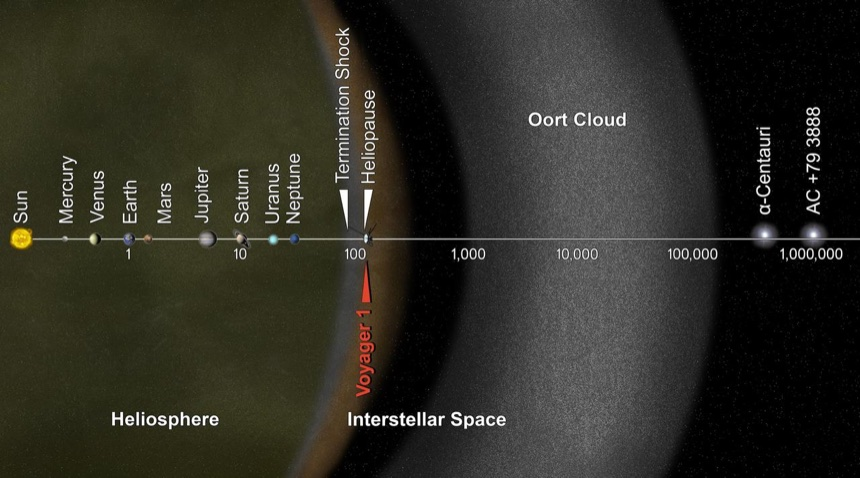
\includegraphics[width=0.78\textwidth,height=5.6cm,keepaspectratio]{../public/textures/nasa/oort_cloud.jpg}\\[3pt]
{\footnotesize\itshape\color{orbitarMuted} Ilustrație științifică oficială NASA/JPL-Caltech (PIA17046): Sfera gigantică de comete înghețate a Norului lui Oort în jurul Sistemului Solar.}
\end{center}


\begin{tcolorbox}[orbitardata, title={\textbf{Repere esențiale: Norul lui Oort}}]
\small
\begin{itemize}[leftmargin=1.4em, itemsep=2pt, topsep=2pt]
  \item \textbf{Clasificare și orbită:} Rezervor Cometar Circumsolar \quad$\bullet$\quad \textbf{Distanță:} aproximativ 1 an-lumină (63.241 UA)
  \item \textbf{Dimensiuni și masă:} Înconjoară întregul Sistem Solar ca o bulă sferică de aproximativ 100.000 de ori mai departe de Soare decât Pământul! \quad$\bullet$\quad masă: 5,000 $\times M_\oplus$
  \item \textbf{Gravitație și regim termic:} Microgravitație / Imponderabilitate ($\approx 0\,g$) \quad$\bullet$\quad temperatură medie: -269 $^\circ$C
  \item \textbf{Ciclu orbital și rotație:} perioadă orbitală (an): 365.250.000 zile ($\approx$ 1000000,00 ani pământești) \quad$\bullet$\quad rotație (zi): 24,00 ore (1,00 zile pământești)
  \item \textbf{Durata călătoriei de pe Pământ:} cu viteza luminii ($1c$): \emph{1 an}; cu racheta ($50.000$ de kilometri pe oră): \emph{21.600 de ani}; cu avionul ($900$ de kilometri pe oră): \emph{1,2 miliarde de ani}; cu mașina ($100$ de kilometri pe oră): \emph{10,8 miliarde de ani}.
  \item \textbf{Repere de scară și curiozitate:} Dacă Pământul ar fi la doar un pas de Soare, Norul lui Oort ar fi un balon uriaș de fulgi de zăpadă aflat la peste 50 de kilometri depărtare! Sondei Voyager 1 îi vor trebui încă 300 de ani doar ca să ajungă la marginea interioară a Norului lui Oort și aproximativ 30.000 de ani ca să îl traverseze complet!
\end{itemize}
\end{tcolorbox}

\vspace{4pt}
\noindent\textbf{Prezentare generală și profil astrofizic.} Norul lui Oort este un rezervor sferic imens de corpuri înghețate (apă, metan, amoniac și monoxid de carbon înghețat), situat între 2.000 și 100.000 UA (aproximativ 1 an-lumină) de Soare. El marchează limita sferei Hill a Sistemului Solar, adică frontiera până la care gravitația Soarelui mai poate reține obiecte pe orbită. La marginea cea mai îndepărtată a Sistemului nostru Solar, acolo unde căldura Soarelui abia se mai simte, plutește o bulă gigantică formată din miliarde de bulgări de gheață și praf cosmic. Acesta este Norul lui Oort, regiunea îndepărtată din care pornesc spre noi cometele cu coadă lungă și strălucitoare! Dacă Pământul ar fi la doar un pas de Soare, Norul lui Oort ar fi un balon uriaș de fulgi de zăpadă aflat la peste 50 de kilometri depărtare!

\medskip
\noindent\textbf{Scara cosmică și călătoria luminii în timp.} La scară astronomică, dimensiunile sale sunt impresionante: Înconjoară întregul Sistem Solar ca o bulă sferică de aproximativ 100.000 de ori mai departe de Soare decât Pământul! Totodată, privind astăzi spre Norul lui Oort, observăm practic trecutul îndepărtat al Universului, întrucât lumina sa a călătorit prin spațiu până la noi: Lumina de la marginea Norului lui Oort călătorește un an întreg până ajunge la ochii noștri pe Pământ!

\medskip
\noindent\textbf{Alcătuirea fizică și structura internă.} Privind în profunzimea sa, alcătuirea fizică este organizată pe mai multe straturi și regiuni distincte, fiecare având un rol bine definit în evoluția și dinamica acestui obiect cosmic. În primul rând se remarcă \textbf{Discul Interior (Norul Hills)}, regiune în formă de tor (2.000 -- 20.000 UA) care alimentează continuu norul exterior cu nuclee cometare. În completarea acestui ansamblu întâlnim \textbf{Sfera Exterioară Oort}, înveliș sferic (20.000 -- 100.000 UA) conținând miliarde de nuclee de comete de perioadă lungă, ușor perturbate de stelele vecine.

\medskip
\noindent\textbf{Observații astronomice și istoricul explorării.} Prezis teoretic de astronomul estonian Ernst Öpik (1932) și de astronomul olandez Jan Oort (1950) pentru a explica de unde vin cometele cu perioade de mii sau milioane de ani. Sondei Voyager 1 îi vor trebui încă 300 de ani doar ca să ajungă la marginea interioară a Norului lui Oort și aproximativ 30.000 de ani ca să îl traverseze complet!

\vspace{6pt}
\begin{tcolorbox}[orbitarquiz, title={\textbf{Întrebare de verificare \#47: Norul lui Oort}}]
\textbf{Ce se găsește în principal în Norul lui Oort, la aproximativ 1 an-lumină de Soare?}
\begin{itemize}[leftmargin=2.2em, itemsep=2pt, topsep=4pt]
  \item[$\square$ \textbf{A.}] Miliarde de nuclee înghețate de comete la granița Sistemului Solar
  \item[$\square$ \textbf{B.}] Planete gazoase fierbinți
  \item[$\square$ \textbf{C.}] Rovere marțiene
  \item[$\square$ \textbf{D.}] Doar sateliți artificiali
\end{itemize}
\vspace{2pt}
{\footnotesize\color{orbitarMuted}\textbf{Răspuns corect:} \textbf{A} (Miliarde de nuclee înghețate de comete la granița Sistemului Solar). \emph{Norul lui Oort este rezervorul sferic uriaș de comete înghețate aflat la limita atracției gravitaționale a Soarelui (aproximativ 1 an-lumină).}}
\end{tcolorbox}
\clearpage


\section{Proxima Centauri \& Proxima b}
\label{sec:body-proxima_centauri}
\vspace{-4pt}
{\large\itshape\color{orbitarAccent} Cea mai apropiată stea de Soare și exoplaneta ei stâncoasă (4,24 ani-lumină)}\\[4pt]


\begin{center}
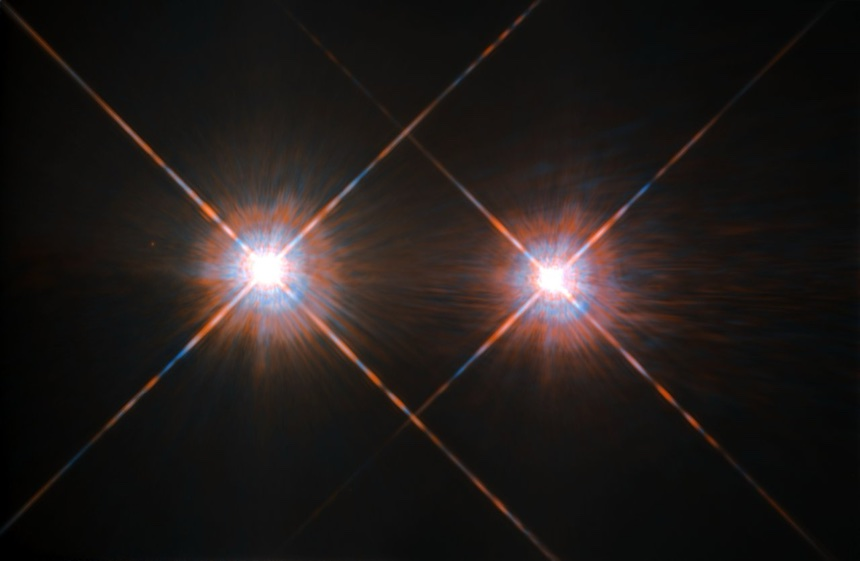
\includegraphics[width=0.78\textwidth,height=5.6cm,keepaspectratio]{../public/textures/nasa/proxima_centauri.jpg}\\[3pt]
{\footnotesize\itshape\color{orbitarMuted} Fotografie reală NASA/ESA (Telescopul Spațial Hubble WFPC2): Steaua pitică roșie Proxima Centauri, aflată la 4,24 ani-lumină.}
\end{center}


\begin{tcolorbox}[orbitardata, title={\textbf{Repere esențiale: Proxima Centauri \& Proxima b}}]
\small
\begin{itemize}[leftmargin=1.4em, itemsep=2pt, topsep=2pt]
  \item \textbf{Clasificare și orbită:} Sistem Exoplanetar / Exoplanetă \quad$\bullet$\quad \textbf{Distanță:} 4,24 ani-lumină
  \item \textbf{Dimensiuni și masă:} Steaua Proxima Centauri are doar 15\% din diametrul Soarelui (cât 1,5 planete Jupiter), iar exoplaneta Proxima b este puțin mai mare decât Pământul (1,07 raze terestre)! \quad$\bullet$\quad masă: 40900,000 $\times M_\oplus$
  \item \textbf{Gravitație și regim termic:} 1,100 $\times g_\oplus$ (10,79 m/s$^2$) \quad$\bullet$\quad temperatură medie: -39 $^\circ$C
  \item \textbf{Ciclu orbital și rotație:} perioadă orbitală (an): 11,186 zile pământești \quad$\bullet$\quad rotație (zi): 268,40 ore (11,18 zile pământești)
  \item \textbf{Durata călătoriei de pe Pământ:} cu viteza luminii ($1c$): \emph{4 ani și 3 luni}; cu racheta ($50.000$ de kilometri pe oră): \emph{75.000 de ani}; cu avionul ($900$ de kilometri pe oră): \emph{5,3 miliarde de ani}; cu mașina ($100$ de kilometri pe oră): \emph{48 de miliarde de ani}.
  \item \textbf{Repere de scară și curiozitate:} Dacă Soarele ar fi un pepene mare și galben, Proxima Centauri ar fi o cireașă roșie strălucitoare, iar planeta Proxima b o bobiță de mazăre care face un tur complet în jurul ei în doar 11 zile! Pe planeta Proxima b, un an întreg durează doar 11 zile pământești! Acolo ai sărbători ziua ta de naștere de trei ori pe lună!
\end{itemize}
\end{tcolorbox}

\vspace{4pt}
\noindent\textbf{Prezentare generală și profil astrofizic.} Situată la 4,24 ani-lumină în constelația Centaurul (parte a sistemului triplu Alpha Centauri), Proxima Centauri este o pitică roșie de clasă spectrală M5.5Ve. Exoplaneta Proxima Centauri b (descoperită în 2016) orbitează chiar în zona locuibilă (la 0,0485 UA de stea), unde temperatura ar permite existența apei lichide. Proxima Centauri este prima noastră vecină stelară din Univers! Este o stea pitică roșie, mai mică și mai blândă decât Soarele, iar în jurul ei se învârte Proxima Centauri b, care este cea mai apropiată exoplanetă (planetă din afara Sistemului Solar) de Pământ! Dacă Soarele ar fi un pepene mare și galben, Proxima Centauri ar fi o cireașă roșie strălucitoare, iar planeta Proxima b o bobiță de mazăre care face un tur complet în jurul ei în doar 11 zile!

\medskip
\noindent\textbf{Scara cosmică și călătoria luminii în timp.} La scară astronomică, dimensiunile sale sunt impresionante: Steaua Proxima Centauri are doar 15\% din diametrul Soarelui (cât 1,5 planete Jupiter), iar exoplaneta Proxima b este puțin mai mare decât Pământul (1,07 raze terestre)! Totodată, privind astăzi spre Proxima Centauri \& Proxima b, observăm practic trecutul îndepărtat al Universului, întrucât lumina sa a călătorit prin spațiu până la noi: Lumina de la Proxima Centauri pe care o vedem azi a plecat acum mai bine de 4 ani și 3 luni, pe când erai cu patru ani mai mic!

\medskip
\noindent\textbf{Alcătuirea fizică și structura internă.} Privind în profunzimea sa, alcătuirea fizică este organizată pe mai multe straturi și regiuni distincte, fiecare având un rol bine definit în evoluția și dinamica acestui obiect cosmic. În primul rând se remarcă \textbf{Steaua Proxima Centauri (M5.5V)}, pitică roșie cu temperatura la suprafață de aproximativ 3.042 K și o durată de viață de mii de miliarde de ani. În strânsă legătură cu această componentă se află \textbf{Exoplaneta Proxima Centauri b}, planetă telurică cu masa minimă de 1,17 mase terestre, orbitând în 11,2 zile în zona locuibilă a stelei. În completarea acestui ansamblu întâlnim \textbf{Proxima Centauri d}, un sub-Pământ foarte apropiat de stea (perioadă orbitală de doar 5,1 zile), descoperit în 2022.

\medskip
\noindent\textbf{Observații astronomice și istoricul explorării.} Steaua a fost descoperită în 1915 de Robert Innes, iar exoplaneta Proxima b a fost confirmată în august 2016 de Observatorul European Austral (ESO) prin metoda vitezelor radiale (instrumentul HARPS). Pe planeta Proxima b, un an întreg durează doar 11 zile pământești! Acolo ai sărbători ziua ta de naștere de trei ori pe lună!

\vspace{6pt}
\begin{tcolorbox}[orbitarquiz, title={\textbf{Întrebare de verificare \#48: Proxima Centauri \& Proxima b}}]
\textbf{La ce distanță de noi se află Proxima Centauri, cea mai apropiată stea de Sistemul Solar?}
\begin{itemize}[leftmargin=2.2em, itemsep=2pt, topsep=4pt]
  \item[$\square$ \textbf{A.}] 4,24 ani-lumină
  \item[$\square$ \textbf{B.}] 100 de kilometri
  \item[$\square$ \textbf{C.}] 2,5 milioane de ani-lumină
  \item[$\square$ \textbf{D.}] 1 Unitate Astronomică
\end{itemize}
\vspace{2pt}
{\footnotesize\color{orbitarMuted}\textbf{Răspuns corect:} \textbf{A} (4,24 ani-lumină). \emph{Proxima Centauri se află la 4,24 ani-lumină (aproximativ 40.000 de miliarde de kilometri) de Sistemul nostru Solar.}}
\end{tcolorbox}
\clearpage


\section{Sirius A \& B (Luceafărul Câinelui)}
\label{sec:body-sirius}
\vspace{-4pt}
{\large\itshape\color{orbitarAccent} Cea mai strălucitoare stea de pe cerul nopții și pitica ei albă (8,6 ani-lumină)}\\[4pt]


\begin{center}
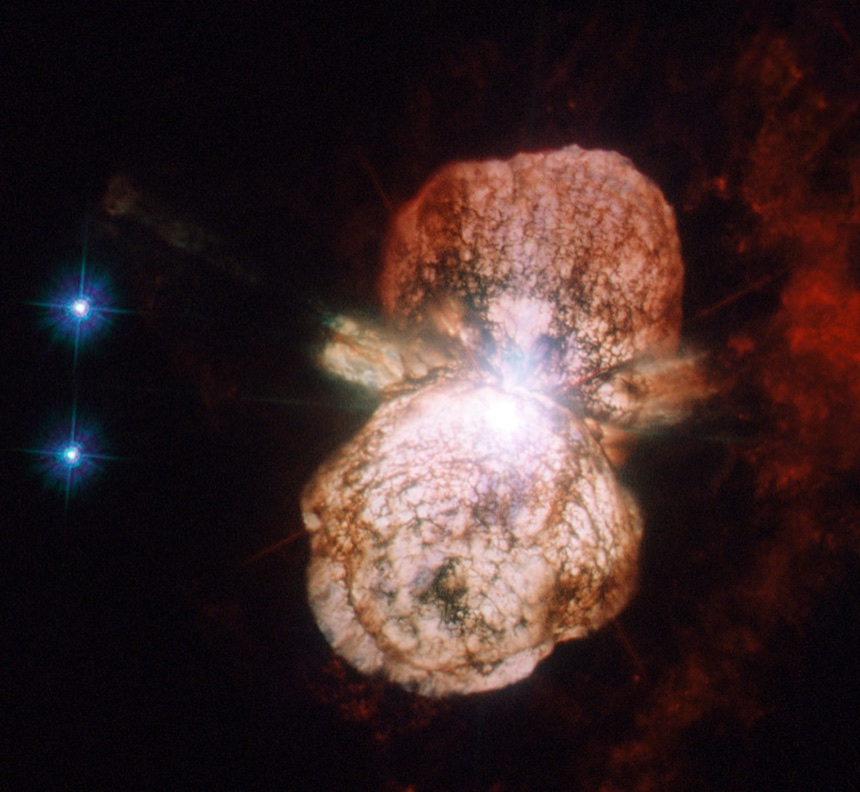
\includegraphics[width=0.78\textwidth,height=5.6cm,keepaspectratio]{../public/textures/nasa/sirius.jpg}\\[3pt]
{\footnotesize\itshape\color{orbitarMuted} Fotografie reală NASA/ESA (Telescopul Spațial Hubble): Steaua strălucitoare Sirius A și pitica albă Sirius B (punctul din stânga-jos).}
\end{center}


\begin{tcolorbox}[orbitardata, title={\textbf{Repere esențiale: Sirius A \& B (Luceafărul Câinelui)}}]
\small
\begin{itemize}[leftmargin=1.4em, itemsep=2pt, topsep=2pt]
  \item \textbf{Clasificare și orbită:} Stea \quad$\bullet$\quad \textbf{Distanță:} 8,6 ani-lumină
  \item \textbf{Dimensiuni și masă:} Sirius A este de 1,71 ori mai mare în diametru decât Soarele și de 25 de ori mai strălucitoare, în timp ce companionul Sirius B (o pitică albă) are masa Soarelui comprimată într-un glob doar cât Pământul! \quad$\bullet$\quad masă: 673000,000 $\times M_\oplus$
  \item \textbf{Gravitație și regim termic:} 22,000 $\times g_\oplus$ (215,82 m/s$^2$) \quad$\bullet$\quad temperatură medie: +9.667 $^\circ$C
  \item \textbf{Ciclu orbital și rotație:} perioadă orbitală (an): 18.299 zile ($\approx$ 50,10 ani pământești) \quad$\bullet$\quad rotație (zi): 16,00 ore (0,67 zile pământești)
  \item \textbf{Durata călătoriei de pe Pământ:} cu viteza luminii ($1c$): \emph{8 ani și 7 luni}; cu racheta ($50.000$ de kilometri pe oră): \emph{154.000 de ani}; cu avionul ($900$ de kilometri pe oră): \emph{10,8 miliarde de ani}; cu mașina ($100$ de kilometri pe oră): \emph{97 de miliarde de ani}.
  \item \textbf{Repere de scară și curiozitate:} Sirius A este ca un far uriaș alb-albăstrui de 25 de ori mai puternic decât Soarele, iar lângă el se rotește Sirius B (\quotedblbase{}Cățelușul\textquotedblright{}), o stea pitică albă mică doar cât Pământul, dar grea cât un Soare întreg! Materia din pitica albă Sirius B este atât de deasă și grea, încât o singură linguriță din ea ar cântări pe Pământ aproximativ 5 tone, adică tot atât cât un elefant african matur!
\end{itemize}
\end{tcolorbox}

\vspace{4pt}
\noindent\textbf{Prezentare generală și profil astrofizic.} Sirius (Alpha Canis Majoris), aflată la 8,6 ani-lumină, este un sistem binar format din Sirius A (stea albă de secvență principală, tip spectral A1V, aproximativ 9.940 K) și Sirius B (una dintre cele mai masive pitice albe cunoscute, cu temperatura de aproximativ 25.000 K), care se orbitează reciproc la fiecare 50,1 ani. Dacă privești cerul senin într-o seară de iarnă, sub centura constelației Orion vei vedea o stea care scânteiază în alb și albastru mai tare decât oricare alta: este Sirius! De fapt, Sirius ascunde un secret fascinant, întrucât nu este o singură stea, ci un sistem binar format din două stele care orbitează împreună! Sirius A este ca un far uriaș alb-albăstrui de 25 de ori mai puternic decât Soarele, iar lângă el se rotește Sirius B (\quotedblbase{}Cățelușul\textquotedblright{}), o stea pitică albă mică doar cât Pământul, dar grea cât un Soare întreg!

\medskip
\noindent\textbf{Scara cosmică și călătoria luminii în timp.} La scară astronomică, dimensiunile sale sunt impresionante: Sirius A este de 1,71 ori mai mare în diametru decât Soarele și de 25 de ori mai strălucitoare, în timp ce companionul Sirius B (o pitică albă) are masa Soarelui comprimată într-un glob doar cât Pământul! Totodată, privind astăzi spre Sirius A \& B (Luceafărul Câinelui), observăm practic trecutul îndepărtat al Universului, întrucât lumina sa a călătorit prin spațiu până la noi: Lumina albastră-albă de la Sirius pe care o vedem în această seară a plecat spre Pământ acum 8,6 ani!

\medskip
\noindent\textbf{Alcătuirea fizică și structura internă.} Privind în profunzimea sa, alcătuirea fizică este organizată pe mai multe straturi și regiuni distincte, fiecare având un rol bine definit în evoluția și dinamica acestui obiect cosmic. În primul rând se remarcă \textbf{Sirius A (Steaua Principală A1V)}, stea alb-albăstruie cu masa de 2,06 mase solare și luminozitate de 25,4 ori mai mare decât a Soarelui. În completarea acestui ansamblu întâlnim \textbf{Sirius B (Pitica Albă DA2)}, nucleu stelar colapsat cu raza de aproximativ 5.840 de kilometri (aproape cât Pământul) și masa de 1,018 mase solare.

\medskip
\noindent\textbf{Observații astronomice și istoricul explorării.} Friedrich Bessel a dedus în 1844 existența unui companion invizibil observând oscilațiile mișcării lui Sirius A, iar Alvan Graham Clark a observat direct pitica albă Sirius B în 1862. Materia din pitica albă Sirius B este atât de deasă și grea, încât o singură linguriță din ea ar cântări pe Pământ aproximativ 5 tone, adică tot atât cât un elefant african matur!

\vspace{6pt}
\begin{tcolorbox}[orbitarquiz, title={\textbf{Întrebare de verificare \#49: Sirius A \& B (Luceafărul Câinelui)}}]
\textbf{Ce tip de stea este companionul Sirius B care orbitează în jurul strălucitoarei Sirius A?}
\begin{itemize}[leftmargin=2.2em, itemsep=2pt, topsep=4pt]
  \item[$\square$ \textbf{A.}] O pitică albă extrem de densă, de mărimea Pământului dar cu masa Soarelui
  \item[$\square$ \textbf{B.}] O planetă de gheață
  \item[$\square$ \textbf{C.}] O supergigantă roșie
  \item[$\square$ \textbf{D.}] Un asteroid metalic
\end{itemize}
\vspace{2pt}
{\footnotesize\color{orbitarMuted}\textbf{Răspuns corect:} \textbf{A} (O pitică albă extrem de densă, de mărimea Pământului dar cu masa Soarelui). \emph{Sirius B este o pitică albă, reprezentând nucleul dens rămas dintr-o stea străveche, având masa Soarelui strânsă într-un volum cât Pământul.}}
\end{tcolorbox}
\clearpage


\section{Sistemul TRAPPIST-1 (7 Exoplanete)}
\label{sec:body-trappist1}
\vspace{-4pt}
{\large\itshape\color{orbitarAccent} Steaua pitică ultra-rece cu 7 planete stâncoase de mărimea Pământului (40 ani-lumină)}\\[4pt]


\begin{center}
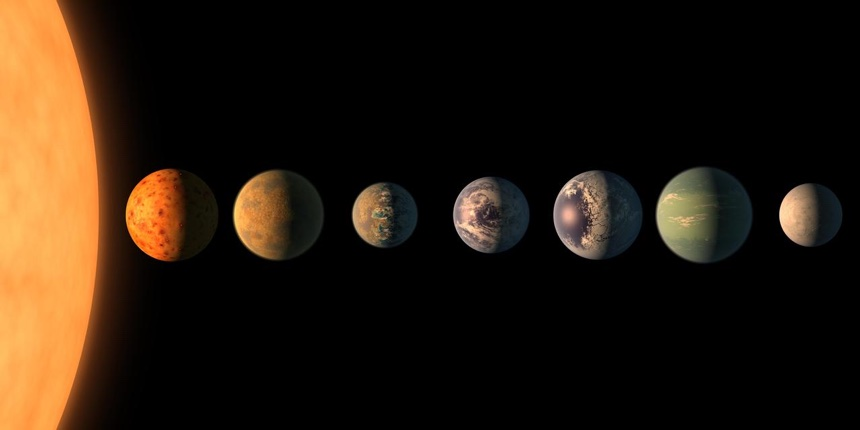
\includegraphics[width=0.78\textwidth,height=5.6cm,keepaspectratio]{../public/textures/nasa/trappist1.jpg}\\[3pt]
{\footnotesize\itshape\color{orbitarMuted} Randare științifică oficială NASA/JPL-Caltech (PIA21422): Cele 7 exoplanete stâncoase de mărimea Pământului din sistemul TRAPPIST-1.}
\end{center}


\begin{tcolorbox}[orbitardata, title={\textbf{Repere esențiale: Sistemul TRAPPIST-1 (7 Exoplanete)}}]
\small
\begin{itemize}[leftmargin=1.4em, itemsep=2pt, topsep=2pt]
  \item \textbf{Clasificare și orbită:} Sistem Exoplanetar / Exoplanetă \quad$\bullet$\quad \textbf{Distanță:} 40 de ani-lumină
  \item \textbf{Dimensiuni și masă:} Steaua TRAPPIST-1 este abia puțin mai mare decât planeta Jupiter (12\% din raza Soarelui), iar toate cele 7 planete ale sale încap pe o orbită mult mai strânsă decât orbita lui Mercur în jurul Soarelui! \quad$\bullet$\quad masă: 29800,000 $\times M_\oplus$
  \item \textbf{Gravitație și regim termic:} 0,930 $\times g_\oplus$ (9,12 m/s$^2$) \quad$\bullet$\quad temperatură medie: -22 $^\circ$C
  \item \textbf{Ciclu orbital și rotație:} perioadă orbitală (an): 6,1 zile pământești \quad$\bullet$\quad rotație (zi): 146,40 ore (6,10 zile pământești)
  \item \textbf{Durata călătoriei de pe Pământ:} cu viteza luminii ($1c$): \emph{40 de ani}; cu racheta ($50.000$ de kilometri pe oră): \emph{720.000 de ani}; cu avionul ($900$ de kilometri pe oră): \emph{50 de miliarde de ani}; cu mașina ($100$ de kilometri pe oră): \emph{450 de miliarde de ani}.
  \item \textbf{Repere de scară și curiozitate:} Dacă Sistemul nostru Solar este un teren mare de fotbal, întregul sistem TRAPPIST-1 cu toate cele 7 planete ale sale ar încăpea în cercul de la mijlocul terenului! Planetele sunt atât de aproape unele de altele, încât de pe una le-ai vedea pe celelalte pe cer mai mari decât vedem noi Luna! Toate cele 7 planete din sistemul TRAPPIST-1 sunt mai aproape de steaua lor decât este Mercur față de Soarele nostru, dar nu se ard fiindcă steaua lor este o pitică ultra-rece și blândă!
\end{itemize}
\end{tcolorbox}

\vspace{4pt}
\noindent\textbf{Prezentare generală și profil astrofizic.} Aflat la aproximativ 40 de ani-lumină în constelația Vărsătorul, sistemul TRAPPIST-1 conține o pitică ultra-rece (clasă M8V, masa aproximativ 0,09 mase solare) și șapte exoplanete telurice (TRAPPIST-1 b, c, d, e, f, g, h) cu perioade orbitale între 1,5 și 18,7 zile, aflate într-un lanț stabil de rezonanțe orbitale. TRAPPIST-1 este unul dintre cele mai uimitoare locuri din galaxie: o stea mică și roșiatică, înconjurată de o familie întreagă de 7 planete stâncoase, toate de mărimea Pământului! Trei dintre aceste planete (e, f și g) se află chiar în \quotedblbase{}zona potrivită\textquotedblright{}, unde ar putea exista oceane de apă lichidă! Dacă Sistemul nostru Solar este un teren mare de fotbal, întregul sistem TRAPPIST-1 cu toate cele 7 planete ale sale ar încăpea în cercul de la mijlocul terenului! Planetele sunt atât de aproape unele de altele, încât de pe una le-ai vedea pe celelalte pe cer mai mari decât vedem noi Luna!

\medskip
\noindent\textbf{Scara cosmică și călătoria luminii în timp.} La scară astronomică, dimensiunile sale sunt impresionante: Steaua TRAPPIST-1 este abia puțin mai mare decât planeta Jupiter (12\% din raza Soarelui), iar toate cele 7 planete ale sale încap pe o orbită mult mai strânsă decât orbita lui Mercur în jurul Soarelui! Totodată, privind astăzi spre Sistemul TRAPPIST-1 (7 Exoplanete), observăm practic trecutul îndepărtat al Universului, întrucât lumina sa a călătorit prin spațiu până la noi: Lumina de la sistemul TRAPPIST-1 pe care o vedem azi a plecat acum 40 de ani (în 1986), pe vremea când părinții tăi erau copii și se lansa stația spațială Mir!

\medskip
\noindent\textbf{Alcătuirea fizică și structura internă.} Privind în profunzimea sa, alcătuirea fizică este organizată pe mai multe straturi și regiuni distincte, fiecare având un rol bine definit în evoluția și dinamica acestui obiect cosmic. În primul rând se remarcă \textbf{Planetele Interioare (b, c, d)}, lumi stâncoase calde studiate în infraroșu de Telescopul Spațial James Webb (JWST) pentru detecția atmosferei. În strânsă legătură cu această componentă se află \textbf{Zona Locuibilă (TRAPPIST-1 e, f, g)}, trei exoplanete de mărimea Pământului aflate la distanța ideală pentru a susține apă lichidă la suprafață. În completarea acestui ansamblu întâlnim \textbf{Planeta Exterioară (TRAPPIST-1 h)}, lume înghețată cu perioada orbitală de 18,77 zile, situată la marginea sistemului compact.

\medskip
\noindent\textbf{Observații astronomice și istoricul explorării.} Descoperit în 2016--2017 de echipa condusă de Michaël Gillon cu telescopul TRAPPIST și telescopul spațial Spitzer; astăzi este ținta principală a Telescopului James Webb pentru studiul atmosferelor exoplanetare. Toate cele 7 planete din sistemul TRAPPIST-1 sunt mai aproape de steaua lor decât este Mercur față de Soarele nostru, dar nu se ard fiindcă steaua lor este o pitică ultra-rece și blândă!

\vspace{6pt}
\begin{tcolorbox}[orbitarquiz, title={\textbf{Întrebare de verificare \#50: Sistemul TRAPPIST-1 (7 Exoplanete)}}]
\textbf{Câte planete stâncoase de mărimea Pământului orbitează în jurul stelei TRAPPIST-1?}
\begin{itemize}[leftmargin=2.2em, itemsep=2pt, topsep=4pt]
  \item[$\square$ \textbf{A.}] 7 exoplanete stâncoase (dintre care 3 în zona locuibilă)
  \item[$\square$ \textbf{B.}] O singură planetă gazoasă
  \item[$\square$ \textbf{C.}] 100 de planete
  \item[$\square$ \textbf{D.}] Nicio planetă
\end{itemize}
\vspace{2pt}
{\footnotesize\color{orbitarMuted}\textbf{Răspuns corect:} \textbf{A} (7 exoplanete stâncoase (dintre care 3 în zona locuibilă)). \emph{Sistemul TRAPPIST-1 deține recordul pentru cele mai multe planete telurice de mărimea Pământului (7 planete: b, c, d, e, f, g, h) în jurul unei singure stele.}}
\end{tcolorbox}
\clearpage


\section{Exoplaneta 55 Cancri e (Janssen)}
\label{sec:body-cancri55e}
\vspace{-4pt}
{\large\itshape\color{orbitarAccent} \quotedblbase{}Planeta de Lavă și Diamant\textquotedblright{}, Super-Pământ incandescent (41 ani-lumină)}\\[4pt]


\begin{center}
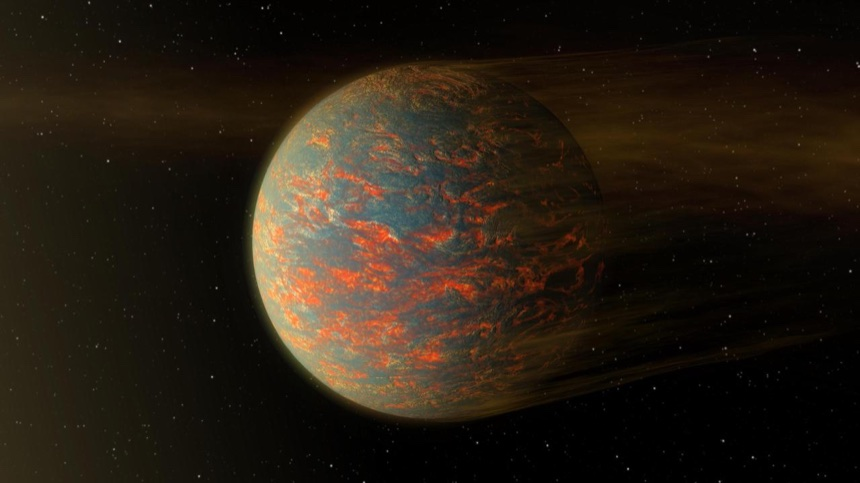
\includegraphics[width=0.78\textwidth,height=5.6cm,keepaspectratio]{../public/textures/nasa/cancri55e.jpg}\\[3pt]
{\footnotesize\itshape\color{orbitarMuted} Imagine științifică oficială NASA/JPL-Caltech (Telescopul Spitzer PIA20068): Exoplaneta incandescentă de lavă 55 Cancri e (Janssen).}
\end{center}


\begin{tcolorbox}[orbitardata, title={\textbf{Repere esențiale: Exoplaneta 55 Cancri e (Janssen)}}]
\small
\begin{itemize}[leftmargin=1.4em, itemsep=2pt, topsep=2pt]
  \item \textbf{Clasificare și orbită:} Sistem Exoplanetar / Exoplanetă \quad$\bullet$\quad \textbf{Distanță:} 41 de ani-lumină
  \item \textbf{Dimensiuni și masă:} Este un \quotedblbase{}Super-Pământ\textquotedblright{} cu diametrul de aproape 2 ori mai mare decât al Pământului și de 8 ori mai masiv! \quad$\bullet$\quad masă: 7,990 $\times M_\oplus$
  \item \textbf{Gravitație și regim termic:} 2,200 $\times g_\oplus$ (21,58 m/s$^2$) \quad$\bullet$\quad temperatură medie: +2.000 $^\circ$C
  \item \textbf{Ciclu orbital și rotație:} perioadă orbitală (an): 0,737 zile pământești \quad$\bullet$\quad rotație (zi): 17,67 ore (0,74 zile pământești)
  \item \textbf{Durata călătoriei de pe Pământ:} cu viteza luminii ($1c$): \emph{41 de ani}; cu racheta ($50.000$ de kilometri pe oră): \emph{738.000 de ani}; cu avionul ($900$ de kilometri pe oră): \emph{51 de miliarde de ani}; cu mașina ($100$ de kilometri pe oră): \emph{460 de miliarde de ani}.
  \item \textbf{Repere de scară și curiozitate:} Dacă Pământul este o bilă albastră acoperită cu oceane de apă răcoroasă, 55 Cancri e este o bilă incandescentă acoperită cu oceane de magmă vulcanică și nori de rocă vaporizată! Pe 55 Cancri e, anul nou vine înainte să se termine o singură zi de pe Pământ: planeta dă ocol stelei sale în doar 17 ore și 40 de minute!
\end{itemize}
\end{tcolorbox}

\vspace{4pt}
\noindent\textbf{Prezentare generală și profil astrofizic.} 55 Cancri e (numită oficial Janssen) este o exoplanetă de tip Super-Pământ aflată la 41 de ani-lumină în constelația Racul. Orbitează la doar 0,015 UA de steaua 55 Cancri A, fiind blocată mareic: emisfera diurnă atinge aproximativ 2.000 $^\circ$C (acoperită de un ocean global de magmă), iar observațiile JWST din 2024 au confirmat prezența unei atmosfere secundare bogate în CO și CO$_2$ degajate din oceanul de lavă. Imaginează-ți o planetă de aproape două ori mai mare decât Pământul, atât de apropiată de steaua ei încât un an întreg acolo durează doar 17 ore și jumătate! Pe partea îndreptată spre stea, stâncile s-au topit într-un ocean uriaș de lavă strălucitoare, iar în adâncuri carbonul presat poate forma straturi întregi de diamant! Dacă Pământul este o bilă albastră acoperită cu oceane de apă răcoroasă, 55 Cancri e este o bilă incandescentă acoperită cu oceane de magmă vulcanică și nori de rocă vaporizată!

\medskip
\noindent\textbf{Scara cosmică și călătoria luminii în timp.} La scară astronomică, dimensiunile sale sunt impresionante: Este un \quotedblbase{}Super-Pământ\textquotedblright{} cu diametrul de aproape 2 ori mai mare decât al Pământului și de 8 ori mai masiv! Totodată, privind astăzi spre Exoplaneta 55 Cancri e (Janssen), observăm practic trecutul îndepărtat al Universului, întrucât lumina sa a călătorit prin spațiu până la noi: Lumina de la sistemul 55 Cancri pe care o vedem azi a plecat acum 41 de ani (în 1985)!

\medskip
\noindent\textbf{Alcătuirea fizică și structura internă.} Privind în profunzimea sa, alcătuirea fizică este organizată pe mai multe straturi și regiuni distincte, fiecare având un rol bine definit în evoluția și dinamica acestui obiect cosmic. În primul rând se remarcă \textbf{Ocean Global de Magmă}, suprafață de silicați topiți pe emisfera diurnă, la temperaturi de peste 2.000 $^\circ$C. În strânsă legătură cu această componentă se află \textbf{Manta Bogată în Carbon și Siliciu}, unde presiunile extreme din interiorul unei planete de 8 mase terestre pot cristaliza carbonul sub formă de diamant. În completarea acestui ansamblu întâlnim \textbf{Atmosferă Volatilă de Roci și Gaze}, atmosferă densă de monoxid și dioxid de carbon detectată de Telescopul Spațial James Webb în 2024.

\medskip
\noindent\textbf{Observații astronomice și istoricul explorării.} Descoperită în 2004 prin metoda vitezelor radiale și observată în tranzit de telescoapele Spitzer, Hubble, CHEOPS și James Webb (2024). Pe 55 Cancri e, anul nou vine înainte să se termine o singură zi de pe Pământ: planeta dă ocol stelei sale în doar 17 ore și 40 de minute!

\vspace{6pt}
\begin{tcolorbox}[orbitarquiz, title={\textbf{Întrebare de verificare \#51: Exoplaneta 55 Cancri e (Janssen)}}]
\textbf{De ce este suprafața exoplanetei 55 Cancri e acoperită de un ocean de lavă topită?}
\begin{itemize}[leftmargin=2.2em, itemsep=2pt, topsep=4pt]
  \item[$\square$ \textbf{A.}] Pentru că orbitează extrem de aproape de steaua ei (un an durează doar aproximativ 18 ore), la aproximativ 2.000 $^\circ$C
  \item[$\square$ \textbf{B.}] Pentru că este făcută din gheață
  \item[$\square$ \textbf{C.}] Pentru că nu are nicio stea în apropiere
  \item[$\square$ \textbf{D.}] Pentru că se află în Centura Kuiper
\end{itemize}
\vspace{2pt}
{\footnotesize\color{orbitarMuted}\textbf{Răspuns corect:} \textbf{A} (Pentru că orbitează extrem de aproape de steaua ei (un an durează doar aproximativ 18 ore), la aproximativ 2.000 $^\circ$C). \emph{Fiind la doar 0,015 UA de steaua ei, 55 Cancri e este încălzită la aproximativ 2.000 $^\circ$C, topind rocile de la suprafață într-un ocean global de magmă.}}
\end{tcolorbox}
\clearpage


\section{Roiul Stelar Pleiadele (\quotedblbase{}Cloșca cu Pui\textquotedblright{})}
\label{sec:body-pleiades}
\vspace{-4pt}
{\large\itshape\color{orbitarAccent} Roiul deschis M45 de stele tinere albastre din Taurul (444 ani-lumină)}\\[4pt]


\begin{center}
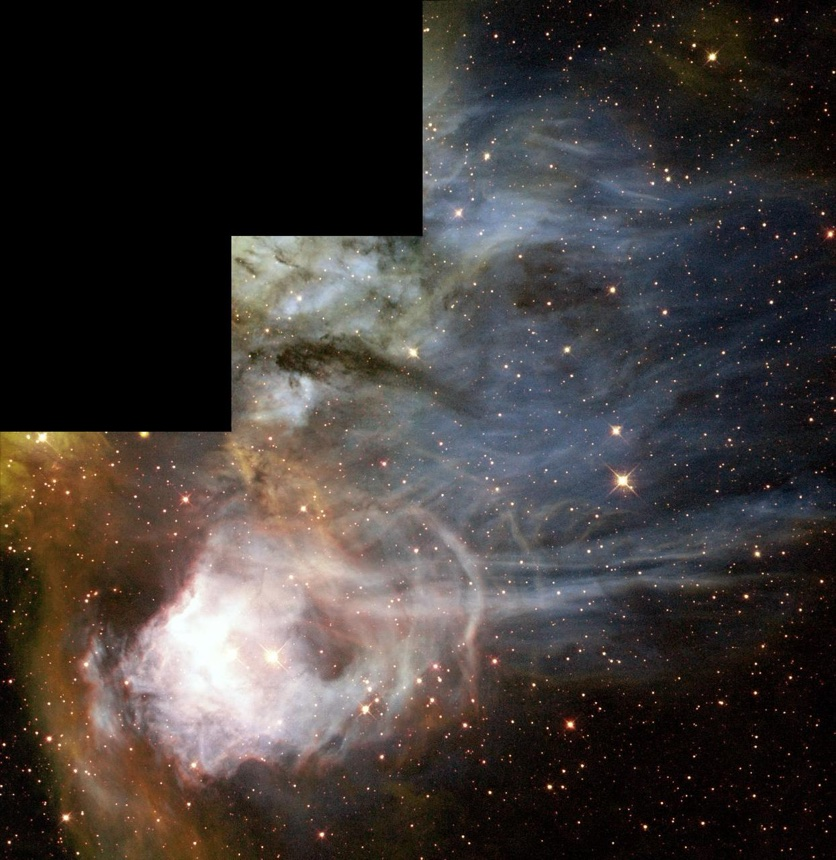
\includegraphics[width=0.78\textwidth,height=5.6cm,keepaspectratio]{../public/textures/nasa/pleiades.jpg}\\[3pt]
{\footnotesize\itshape\color{orbitarMuted} Fotografie reală NASA/JPL-Caltech/Hubble (PIA04225): Roiul stelar deschis Pleiadele (M45, \quotedblbase{}Cloșca cu Pui\textquotedblright{}).}
\end{center}


\begin{tcolorbox}[orbitardata, title={\textbf{Repere esențiale: Roiul Stelar Pleiadele (\quotedblbase{}Cloșca cu Pui\textquotedblright{})}}]
\small
\begin{itemize}[leftmargin=1.4em, itemsep=2pt, topsep=2pt]
  \item \textbf{Clasificare și orbită:} Roi Stelar Deschis \quad$\bullet$\quad \textbf{Distanță:} 444 de ani-lumină
  \item \textbf{Dimensiuni și masă:} Roiul Pleiadelor conține peste 1.000 de stele tinere răspândite pe o lățime de aproximativ 17 ani-lumină (de 17 ori mai mare decât întregul Nor al lui Oort)! \quad$\bullet$\quad masă: 266000000,000 $\times M_\oplus$
  \item \textbf{Gravitație și regim termic:} 1,000 $\times g_\oplus$ (9,81 m/s$^2$) \quad$\bullet$\quad temperatură medie: +12.000 $^\circ$C
  \item \textbf{Ciclu orbital și rotație:} perioadă orbitală (an): Orbitează centrul Căii Lactee (aproximativ 230 de milioane de ani) \quad$\bullet$\quad rotație (zi): 24,00 ore (1,00 zile pământești)
  \item \textbf{Durata călătoriei de pe Pământ:} cu viteza luminii ($1c$): \emph{444 de ani}; cu racheta ($50.000$ de kilometri pe oră): \emph{8 milioane de ani}; cu avionul ($900$ de kilometri pe oră): \emph{550 de miliarde de ani}; cu mașina ($100$ de kilometri pe oră): \emph{5.000 de miliarde de ani}.
  \item \textbf{Repere de scară și curiozitate:} Pleiadele sunt ca o \quotedblbase{}grădiniță de stele-frați\textquotedblright{} născute din același nor cosmic acum 100 de milioane de ani, în epoca în care pe Pământ încă trăiau dinozaurii! Lumina albastră de la \quotedblbase{}Cloșca cu Pui\textquotedblright{} călătorește prin spațiu timp de 444 de ani până ajunge la noi: razele pe care le vezi diseară au plecat de acolo pe vremea lui Mihai Viteazul!
\end{itemize}
\end{tcolorbox}

\vspace{4pt}
\noindent\textbf{Prezentare generală și profil astrofizic.} Pleiadele (Messier 45 / \quotedblbase{}Cloșca cu Pui\textquotedblright{}), situate la aproximativ 444 de ani-lumină în constelația Taurul, reprezintă cel mai cunoscut roi stelar deschis de pe cer. Este dominat de gigante albastre extrem de luminoase (Alcyone, Atlas, Electra, Maia, Merope, Taygeta, Pleione) care iluminează o nebuloasă de reflexie albastră la trecerea printr-un nor interstelar de praf. Când privești cerul nopții toamna sau iarna, poți vedea cu ochiul liber un buchet mic și sclipitor de 7 stele albastre care stau strânse împreună. În România, bunicii noștri le-au numit cu drag \quotedblbase{}Cloșca cu Pui\textquotedblright{} sau \quotedblbase{}Găinușa\textquotedblright{}! Prin telescop însă descoperim că acolo sunt peste 1.000 de stele tinere și fierbinți, învăluite într-un voal albastru de praf stelar! Pleiadele sunt ca o \quotedblbase{}grădiniță de stele-frați\textquotedblright{} născute din același nor cosmic acum 100 de milioane de ani, în epoca în care pe Pământ încă trăiau dinozaurii!

\medskip
\noindent\textbf{Scara cosmică și călătoria luminii în timp.} La scară astronomică, dimensiunile sale sunt impresionante: Roiul Pleiadelor conține peste 1.000 de stele tinere răspândite pe o lățime de aproximativ 17 ani-lumină (de 17 ori mai mare decât întregul Nor al lui Oort)! Totodată, privind astăzi spre Roiul Stelar Pleiadele (\quotedblbase{}Cloșca cu Pui\textquotedblright{}), observăm practic trecutul îndepărtat al Universului, întrucât lumina sa a călătorit prin spațiu până la noi: Lumina de la Pleiade (\quotedblbase{}Cloșca cu Pui\textquotedblright{}) pe care o vedem azi pe cer a plecat acum 444 de ani, în anul 1582, pe vremea lui Mihai Viteazul!

\medskip
\noindent\textbf{Alcătuirea fizică și structura internă.} Privind în profunzimea sa, alcătuirea fizică este organizată pe mai multe straturi și regiuni distincte, fiecare având un rol bine definit în evoluția și dinamica acestui obiect cosmic. În primul rând se remarcă \textbf{Cele 7 Surori (Gigante Albastre B)}, stele masive și tinere (aproximativ 100 de milioane de ani), fiecare de sute de ori mai luminoasă decât Soarele. În completarea acestui ansamblu întâlnim \textbf{Nebuloasa de Reflexie Merope (NGC 1435)}, nor fin de praf interstelar care împrăștie lumina albastră a stelelor din roi.

\medskip
\noindent\textbf{Observații astronomice și istoricul explorării.} Cunoscute din antichitate în toate culturile lumii (și în astronomia populară românească drept \quotedblbase{}Cloșca cu Pui\textquotedblright{}), Pleiadele au fost desenate pentru prima dată prin telescop de Galileo Galilei în 1610 și catalogate de Charles Messier ca M45 în 1769. Lumina albastră de la \quotedblbase{}Cloșca cu Pui\textquotedblright{} călătorește prin spațiu timp de 444 de ani până ajunge la noi: razele pe care le vezi diseară au plecat de acolo pe vremea lui Mihai Viteazul!

\vspace{6pt}
\begin{tcolorbox}[orbitarquiz, title={\textbf{Întrebare de verificare \#52: Roiul Stelar Pleiadele (\quotedblbase{}Cloșca cu Pui\textquotedblright{})}}]
\textbf{Cum este numit roiul stelar Pleiadele (M45) în tradiția populară românească și acum câți ani a plecat lumina lui spre noi?}
\begin{itemize}[leftmargin=2.2em, itemsep=2pt, topsep=4pt]
  \item[$\square$ \textbf{A.}] \quotedblbase{}Cloșca cu Pui\textquotedblright{}, iar lumina a plecat acum aproximativ 444 de ani
  \item[$\square$ \textbf{B.}] \quotedblbase{}Carul Mare\textquotedblright{}, la 10 kilometri distanță
  \item[$\square$ \textbf{C.}] \quotedblbase{}Luceafărul de Dimineață\textquotedblright{}, la 8 minute-lumină
  \item[$\square$ \textbf{D.}] \quotedblbase{}Calea Robilor\textquotedblright{}, la 1 miliard de ani-lumină
\end{itemize}
\vspace{2pt}
{\footnotesize\color{orbitarMuted}\textbf{Răspuns corect:} \textbf{A} (\quotedblbase{}Cloșca cu Pui\textquotedblright{}, iar lumina a plecat acum aproximativ 444 de ani). \emph{În tradiția românească, Pleiadele sunt numite \quotedblbase{}Cloșca cu Pui\textquotedblright{} (sau \quotedblbase{}Găinușa\textquotedblright{}), iar la distanța de 444 de ani-lumină, lumina lor a plecat spre Pământ în secolul al XVI-lea.}}
\end{tcolorbox}
\clearpage


\section{Betelgeuse (Supergiganta Roșie)}
\label{sec:body-betelgeuse}
\vspace{-4pt}
{\large\itshape\color{orbitarAccent} Steaua colosală din Orion, de aproximativ 700 de ori mai mare decât Soarele (640 ani-lumină)}\\[4pt]


\begin{center}
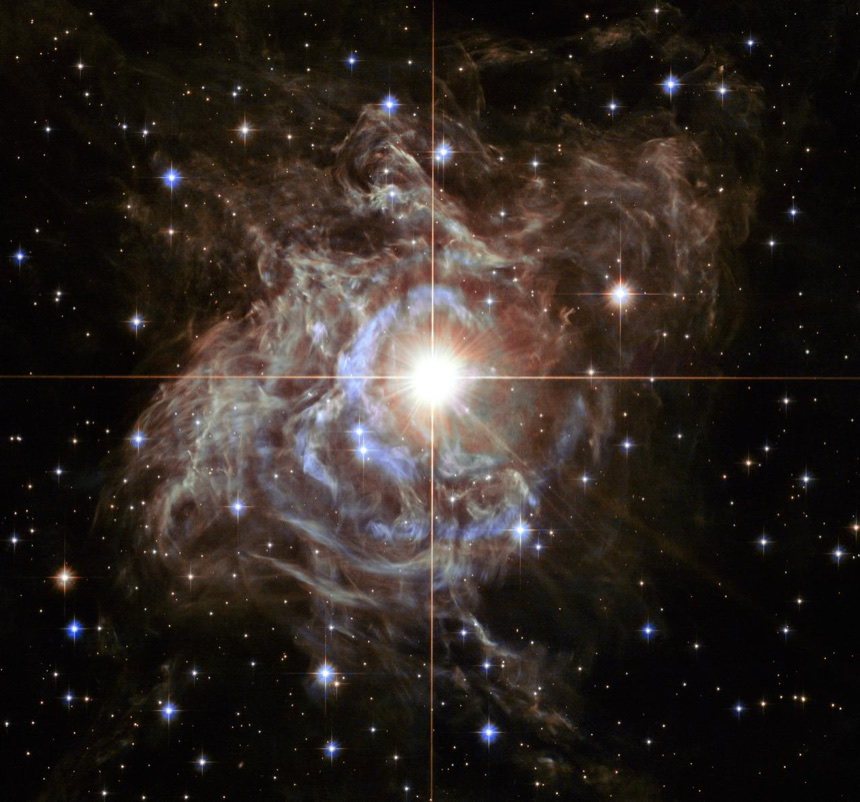
\includegraphics[width=0.78\textwidth,height=5.6cm,keepaspectratio]{../public/textures/nasa/betelgeuse.jpg}\\[3pt]
{\footnotesize\itshape\color{orbitarMuted} Imagine reală NASA/ESA (Telescopul Spațial Hubble): Supergiganta roșie Betelgeuse din constelația Orion.}
\end{center}


\begin{tcolorbox}[orbitardata, title={\textbf{Repere esențiale: Betelgeuse (Supergiganta Roșie)}}]
\small
\begin{itemize}[leftmargin=1.4em, itemsep=2pt, topsep=2pt]
  \item \textbf{Clasificare și orbită:} Stea \quad$\bullet$\quad \textbf{Distanță:} 640 de ani-lumină
  \item \textbf{Dimensiuni și masă:} Betelgeuse are un diametru de aproximativ 700 de ori mai mare decât Soarele! Dacă am așeza-o în centrul Sistemului Solar, marginea ei ar înghiți Mercur, Venus, Pământul, Marte și ar ajunge până la orbita lui Jupiter! \quad$\bullet$\quad masă: 5500000,000 $\times M_\oplus$
  \item \textbf{Gravitație și regim termic:} Microgravitație / Imponderabilitate ($\approx 0\,g$) \quad$\bullet$\quad temperatură medie: +3.327 $^\circ$C
  \item \textbf{Ciclu orbital și rotație:} perioadă orbitală (an): Orbitează centrul Căii Lactee (aproximativ 230 de milioane de ani) \quad$\bullet$\quad rotație (zi): 720,00 ore (30,00 zile pământești)
  \item \textbf{Durata călătoriei de pe Pământ:} cu viteza luminii ($1c$): \emph{640 de ani}; cu racheta ($50.000$ de kilometri pe oră): \emph{11,5 milioane de ani}; cu avionul ($900$ de kilometri pe oră): \emph{800 de miliarde de ani}; cu mașina ($100$ de kilometri pe oră): \emph{7.200 de miliarde de ani}.
  \item \textbf{Repere de scară și curiozitate:} Dacă Soarele nostru ar fi o minge mică de ping-pong, supergiganta Betelgeuse ar fi un balon gonflabil înalt cât o clădire cu 9 etaje (28 de metri diametru)! În anul 2019, Betelgeuse s-a întunecat brusc pentru câteva luni, iar astronomii au descoperit cu telescopul Hubble că steaua \quotedblbase{}strănutase\textquotedblright{} un nor uriaș de praf cosmic care îi umbrea fața!
\end{itemize}
\end{tcolorbox}

\vspace{4pt}
\noindent\textbf{Prezentare generală și profil astrofizic.} Betelgeuse (Alpha Orionis), aflată la aproximativ 640 de ani-lumină, este o supergigantă roșie variabilă semiregulată (clasă spectrală M1--M2 Ia-ab) aflată în ultimele etape ale evoluției sale stelare. Cu o rază de aproximativ 700 raze solare și o luminozitate de aproximativ 100.000 de ori mai mare decât a Soarelui, Betelgeuse își fuzionează elementele grele din nucleu și va sfârși într-o supernovă spectaculoasă în următorii aproximativ 100.000 de ani. În umărul stâng al constelației Orion strălucește o stea portocalie-roșiatică de o mărime aproape de neimaginat: Betelgeuse! Este o supergigantă roșie atât de uriașă, încât înăuntrul ei ar încăpea sute de milioane de Sori! Dacă Betelgeuse ar fi pusă în locul Soarelui nostru, Pământul și chiar Marte s-ar afla în interiorul stelei! Dacă Soarele nostru ar fi o minge mică de ping-pong, supergiganta Betelgeuse ar fi un balon gonflabil înalt cât o clădire cu 9 etaje (28 de metri diametru)!

\medskip
\noindent\textbf{Scara cosmică și călătoria luminii în timp.} La scară astronomică, dimensiunile sale sunt impresionante: Betelgeuse are un diametru de aproximativ 700 de ori mai mare decât Soarele! Dacă am așeza-o în centrul Sistemului Solar, marginea ei ar înghiți Mercur, Venus, Pământul, Marte și ar ajunge până la orbita lui Jupiter! Totodată, privind astăzi spre Betelgeuse (Supergiganta Roșie), observăm practic trecutul îndepărtat al Universului, întrucât lumina sa a călătorit prin spațiu până la noi: Lumina roșiatică de la Betelgeuse pe care o vedem azi a plecat acum 640 de ani, în anul 1386, chiar în anul în care a început domnia lui Mircea cel Bătrân în Țara Românească!

\medskip
\noindent\textbf{Alcătuirea fizică și structura internă.} Privind în profunzimea sa, alcătuirea fizică este organizată pe mai multe straturi și regiuni distincte, fiecare având un rol bine definit în evoluția și dinamica acestui obiect cosmic. În primul rând se remarcă \textbf{Fotosferă Convectivă Uriașă}, celule gigantice de convecție (fiecare cât orbita Pământului) care fac suprafața stelei să pulseze și să își schimbe strălucirea. În completarea acestui ansamblu întâlnim \textbf{Înveliș Circumstelar de Praf}, nori extinși de silicați și alumină expulzați de vântul stelar puternic până la zeci de raze stelare.

\medskip
\noindent\textbf{Observații astronomice și istoricul explorării.} În 1920, Betelgeuse a devenit prima stea (în afară de Soare) al cărei diametru unghiular a fost măsurat direct (de Michelson și Pease la Observatorul Mount Wilson); în 2019--2020 a trecut prin \quotedblbase{}Marea Întunecare\textquotedblright{} studiată de Hubble și VLT. În anul 2019, Betelgeuse s-a întunecat brusc pentru câteva luni, iar astronomii au descoperit cu telescopul Hubble că steaua \quotedblbase{}strănutase\textquotedblright{} un nor uriaș de praf cosmic care îi umbrea fața!

\vspace{6pt}
\begin{tcolorbox}[orbitarquiz, title={\textbf{Întrebare de verificare \#53: Betelgeuse (Supergiganta Roșie)}}]
\textbf{Până unde s-ar întinde supergiganta roșie Betelgeuse dacă ar fi așezată în locul Soarelui nostru?}
\begin{itemize}[leftmargin=2.2em, itemsep=2pt, topsep=4pt]
  \item[$\square$ \textbf{A.}] Ar înghiți Mercur, Venus, Pământul și Marte, ajungând aproape de orbita lui Jupiter
  \item[$\square$ \textbf{B.}] Ar fi mai mică decât Luna
  \item[$\square$ \textbf{C.}] Ar ajunge doar până la Stația Spațială Internațională
  \item[$\square$ \textbf{D.}] Ar fi de mărimea unui asteroid
\end{itemize}
\vspace{2pt}
{\footnotesize\color{orbitarMuted}\textbf{Răspuns corect:} \textbf{A} (Ar înghiți Mercur, Venus, Pământul și Marte, ajungând aproape de orbita lui Jupiter). \emph{Având o rază de aproximativ 700 de ori mai mare decât a Soarelui (aproximativ 3,5 UA), Betelgeuse ar depăși orbita lui Marte și Centura de Asteroizi, apropiindu-se de Jupiter.}}
\end{tcolorbox}
\clearpage

